\chapter{Anwendung zur TLS-Simulation}
\label{cha_implementation}

Im folgenden Kapitel wird nun auf die im Rahmen dieser Arbeit entwickelte Anwendung eingegangen. 
Die Anwendung ist speziell für den Einsatz in der Hochschullehre gedacht und soll dazu dienen Protokolle und ihre internen Abläufe darzustellen und durch zusätzliche Interaktivität exploratives Lernen zu ermöglichen. Eine Vorgabe war die Möglichkeit der Erweiterbarkeit der Anwendung um weitere Protokolle. \\
Im ersten Abschnitt werden allgemeine Entscheidungen erläutert, die getroffen wurden, um diese Vorgabe zu ermöglichen. Außerdem werden Überlegungen für die Erweiterung der Anwendung um das TLS-Protokoll dargelegt.\\
Danach wird die Implementation beschrieben, wobei zuerst auf die Umsetzung der allgemeinen Anwendung eingegangen wird und danach auf die konkrete Umsetzung des TLS-Protokolls.

Anschließend werden anhand eines Beispiels einige Hinweise gegeben, was bei der Erweiterung der Anwendung um weitere Protokolle zu beachten ist.

\section{Analyse und Entwurf}

\subsection{Abstrakter Rahmen für die Anwendung}

Um die Vorgabe der Erweiterbarkeit der Anwendung zu ermöglichen, wurden zu Beginn der Entwicklungsarbeit die Gemeinsamkeiten von Protokollen herausgearbeitet, um diese abstrakt umsetzen zu können. So müssen anschließend lediglich protokollspezifische Eigenschaften in Erweiterungen implementiert werden.\\
Die Anwendung soll sich auf Protokolle mit zwei Parteien beschränken. Zwischen diesen Parteien werden Nachrichten eines festen Formats (sogenannte Protokolldateneinheiten) über einen Kanal ausgetauscht. Die Abfolge verschiedener Nachrichtentypen und die bei ihrem Empfang stattfindenden Verarbeitungsschritte sind durch das Protokoll festgelegt. Zusätzlich besitzen die Parteien einen internen Zustand\footnote{
	Um Verwechslungen mit den im nächsten Absatz eingeführten Automatenzuständen zu vermeiden, wird der Zustand einer Partei im Folgenden immer als interner Zustand bezeichnet.
}, der beispielsweise als Resultat empfangener Nachrichten verändert werden kann. 

Aus diesen Voraussetzungen wurde ein abstrakter Rahmen entwickelt, der für konkrete Protokolle erweitert werden muss.
Für ein Protokoll sollte eine Art von Nachrichten bestehen, die von den Parteien gesendet und empfangen werden kann. Dazu muss ein Kanal zwischen den Parteien bestehen, über den das Senden geschehen kann.\\
Um die Parteien, ihre internen Zustände und die Verarbeitungsschritte bei Nachrichtenempfang strukturiert entwickeln zu können, werden die Parteien als endliche Automaten betrachtet. Es können verschiedene Zustände implementiert werden, um strukturiert unterschiedliches Verhalten bei dem Erhalt von Nachrichten zu erlangen. Der Automat besitzt jeweils immer genau einen aktuellen Zustand, an den eingehende Nachrichten weitergeleitet werden. Abhängig vom gewünschten Verhalten können aus dem aktuellen Zustand heraus der aktuelle Zustand neu gesetzt und Nachrichten gesendet werden. Der Automat kann seinen Zuständen zusätzlich Zugriff auf den internen Zustand der Partei bereitstellen.

\begin{figure}
	\centering
	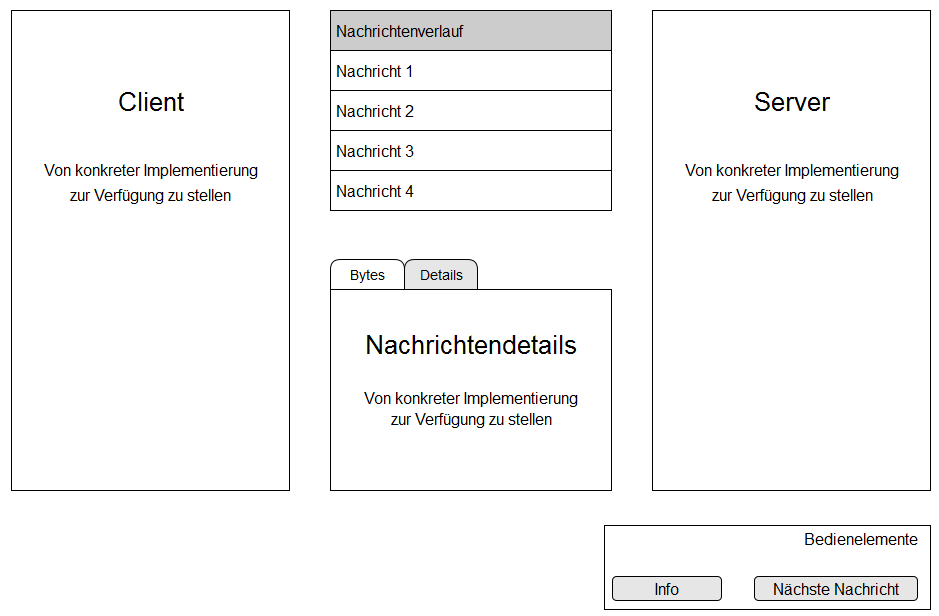
\includegraphics[width=15cm]{Diagrams/SketchUI.png} %
	\caption{Prototyp für die Benutzeroberfläche}
	\label{fig_ui_sketch}
\end{figure}

Anschließend wurde prototypisch eine Benutzeroberfläche entwickelt, die auf Basis dieser Überlegungen auch einen visuellen Rahmen bereitstellt, der für konkrete Protokolle gefüllt werden kann. Ein Prototyp ist in Abbildung\ref{fig_ui_sketch} zu sehen. Es musste möglich sein, den internen Zustand der beiden Parteien darzustellen, der jedoch vom betrachteten Protokoll abhängig ist. Ebenso sollte zu jeder protokollabhängigen Nachricht neben ihrer reinen Repräsentation als Bytefolge auch noch eine Möglichkeit angeboten werden ihre Bedeutung darzustellen. Zusätzlich sollte es möglich sein, dem Verlauf des Protokoll schrittweise zu folgen, um ablaufende Prozesse und Veränderungen an den internen Zuständen zu erkennen. Für das Verständnis von Protokollverhalten bei (absichtlich oder unabsichtlich) veränderten Nachrichten wäre auch eine Möglichkeit für das Bearbeiten von Nachrichten sinnvoll.\\
Mit diesen Möglichkeiten werden auch die Forderungen an exploratives Lernen und Simulationen aus Abschnitt \ref{sec_exploration}, insbesondere der Sichtenwechsel, die Anzeige nicht sichtbarer Prozesse und die Interaktivität, erfüllt.

\subsection{Erweiterung der Anwendung um TLS 1.2}

Für diese Arbeit wurde die TLS 1.2-Spezifikation als Erweiterung des abstrakten Rahmens umgesetzt. Hierdurch lässt sich die zum jetzigen Zeitpunkt aktuelle Version explorieren und insbesondere Abwehrmechanismen gegen Angriffe auf ältere Protokollversionen erkennen. Um diese Angriffe beobachten zu können, hätte sich auch eine ältere Protokollversion wie SSL 2.0 angeboten. Durch die Erweiterbarkeit der Anwendung wäre dieses eine Möglichkeit für spätere Arbeiten.

Im ersten Schritt wurden für Client und Server auf Basis der TLS-Spezifikation Automatenmodelle entwickelt, die abhängig von empfangenen Nachrichten Zustandswechsel und gesendete Nachrichten abbilden. Die Modelle sind im Anhang \ref{cha_tls_state_machines} zu finden. An den Zustandsübergängen sind jeweils die empfangenen Nachrichten in orange dargestellt, die zu diesem Übergang führen. Ist keine Nachricht angegeben, so findet direkt nach Eintritt in den Zustand der Zustandswechsel statt. Mit OnEnter gekennzeichnete Kästen an Zuständen zeigen in blau Nachrichten, die gesendet werden sollen, wenn ein Zustand aktueller Zustand wird. Kästen an Zustandsübergängen stehen für Aktionen, die von außen von dem Automaten verlangt werden (beispielsweise ein Verbindungsaufbauwunsch). In diese Kästen werden zu sendende Nachrichten ebenfalls in blau dargestellt. In eckigen Klammern werden Bedingungen für Zustandsübergänge und andere Aktionen angegeben. Der Startzustand wird durch die Unterstreichung des Namens gekennzeichnet.
 
Danach wurde eine einfache Möglichkeit für die Darstellung der internen Zustände von Server und Client, sowie für die Bedeutungsdarstellung von Nachrichten ausgearbeitet. Hierbei sollten insbesondere auch die Zustandsveränderungen kenntlich gemacht werden, um abgelaufene Vorgänge zu verdeutlichen. Die Wahl fiel auf eine baumartige Struktur aus Objekten, denen ein Titel und ein Wert sowie eine optionale Liste von Kindelementen zugewiesen werden kann. Veränderungen zwischen zwei Zuständen sollten durch Kennzeichnung der geänderten Objekte geschehen.

% Tls 1.2 nicht implementiert

Anschließend wurde die TLS-Spezifikation auf Funktionen untersucht, die nicht implementiert werden sollten. Dies geschah aus Gründen der Komplexitätsreduktion zum besseren Verständnis oder schlicht aus Zeitgründen, insbesondere wenn die Funktion wenig zum Verständnis beigetragen hätte. Im Folgenden soll kurz auf diese Funktionen und auf die Gründe, aus denen sie ausgelassen wurden, eingegangen werden.\\
Auf TLS-Extensions wurde komplett verzichtet, da sie nicht für das grundsätzliche Verständnis von TLS notwendig sind, sondern eher technische Erweiterungen des Standards darstellen, um bestimmte Funktionen nachzurüsten oder Verhalten zu erzwingen.\\
Auch die Möglichkeit TLS-Plaintexte vor dem Verschlüsseln zu komprimieren wurde nicht implementiert, da die Funktion wenig zum Verständnis beiträgt und zusätzlich aufgrund ihrer Angreifbarkeit in der nächsten Protokollversion nicht mehr enthalten sein wird (vgl. Abschnitt \ref{sec_attack_crime}).\\
TLS unterstützt optional zusätzliche Clientauthentifizierung. Diese wird allerdings in vielen Anwendungsfällen, wie beim dem verschlüsselten Abruf einer Internetseite über HTTPS, nicht genutzt und unterscheidet sich prinzipiell nicht übermäßig von der Serverauthentifizierung. Daher wurde in der Anwedung darauf verzichtet.\\
Weiterhin wurden nur einige \ciphersuites implementiert. Hierbei wurde jedoch darauf geachtet, dass sowohl Block- und AEAD-Chiffren zur Ver- und Entschlüsselung als auch RSA und das Diffie-Hellman-Verfahren zum Schlüsselaustausch verwendet wurden. Auf die Implementierung von \ciphersuites, die sich lediglich in Schlüssellängen von bereits implementierten \ciphersuites unterscheiden oder deren Chiffren bzw. Schlüsselaustauschalgorithmen bereits durch andere \ciphersuites abgedeckt waren, wurde bewusst verzichtet. Aus Zeitgründen und da von der Verwendung bereits abgeraten wird, wurde auch auf die Implementierung einer \ciphersuite{} mit der Stromchiffre RC4 verzichtet.\\
Auch die sichere Verwaltung von Schlüsseln im Dateisystem, sowie die Entfernung verwendeter Schlüssel aus dem Speicher, auf die in produktiv verwendeten Systemen geachtet werden muss, wurde hier aus naheliegenden Gründen vernachlässigt.\\
Aus Zeitgründen wurde auch auf die Wiederaufnahme bestehender Sitzungen verzichtet (siehe Abschnitt \ref{sec_session_connection}). Der verkürzte Handshake hat eher praktische Bedeutung, da auf erneute Aushandlung kryptographischer Verfahren und damit mehrere Nachrichten während des Handshakes verzichtet werden kann und die Wiederaufnahme der Verbindung somit weniger Zeit in Anspruch nimmt. Eine spätere Erweiterung der Anwedung um diese Funktion wäre jedoch sinnvoll, um das Verständnis von TLS zu vertiefen.\\
Ein letzter Punkt, der in der Anwedung nicht implementiert wurde, ist die Zertifikatsvalidierung. Diese ist zwar entscheidend für den sicheren Aufbau einer Verbindung, hat aber eher indirekt mit der der Protokollspezifikation zu tun. Daher wurde aus Zeitgründen auf diese Funktion verzichtet, die sich jedoch für spätere Arbeiten anbieten würde.

\section{Implementierung}

Die Wahl der Programmiersprache für die Anwendung fiel auf Java, da diese Sprache an der Universität Hamburg in der ersten Semestern zum Einsatz kommt und von den Studierenden zwingend gelernt werden muss. Auf diese Weise sollte die entwickelte Anwendung auch von anderen Studierenden erweitert oder zumindest problemlos verstanden werden können. Zur Erzeugung der Benutzeroberfläche wurde die in der Java-Runtime verfügbare Bibliothek Swing genutzt, da diese ebenfalls in einigen Veranstaltungen an der Universität Hamburg verwendet wird.

\subsection{Abstrakter Rahmen für die Anwendung}

% abstract model
Ein UML-Diagramm der entwickelten Klassen für den abstrakten Rahmen ist in Abbildung \ref{fig_uml_abstract_state_machine} zu finden. Im Folgenden werden diese Klassen im Detail betrachtet.

Protokollnachrichten werden durch die abstrakte Klasse \sourceobject{ProtocolDataUnit} dargestellt. In Unterklassen muss die Byte-Repräsentation einer Nachricht sowie Titel und Untertitel für die Darstellung auf der Benutzeroberfläche implementiert werden.

Für den abstrakten Rahmen wurden die Parteien als endliche Automaten modelliert. Für diese Modellierung wird das Entwurfsmuster Zustand verwendet. Details hierzu sind \cite{freeman04} zu entnehmen.\\
Die abstrakte Klasse \sourceobject{StateMachine} bildet das Grundgerüst für einen Automaten und die abstrakte Klasse \sourceobject{State} wird zur Implementierung der jeweiligen Automatenzustände verwendet. In einem \sourceobject{StateMachine}-Objekt kann der aktuelle Zustand gesetzt und abgefragt, sowie Nachrichten gesendet werden. Die möglichen Zustände müssen dem Objekt vorher mitgeteilt werden. Zur Beobachtung von Zustandsänderungen wird das Beobachter-Muster verwendet. Dieses Entwurfsmuster ist ebenfalls in \cite{freeman04} zu finden.\\
Unterklassen von \sourceobject{State} implementieren das Verhalten bei Empfang einer Nachricht und bei Betreten und Verlassen des Zustand. Außerdem ermöglichen sie das Senden von Nachrichten und das Setzen des aktuellen Zustands des besitzenden \sourceobject{StateMachine}-Objekts.

\begin{figure}
	\centering
	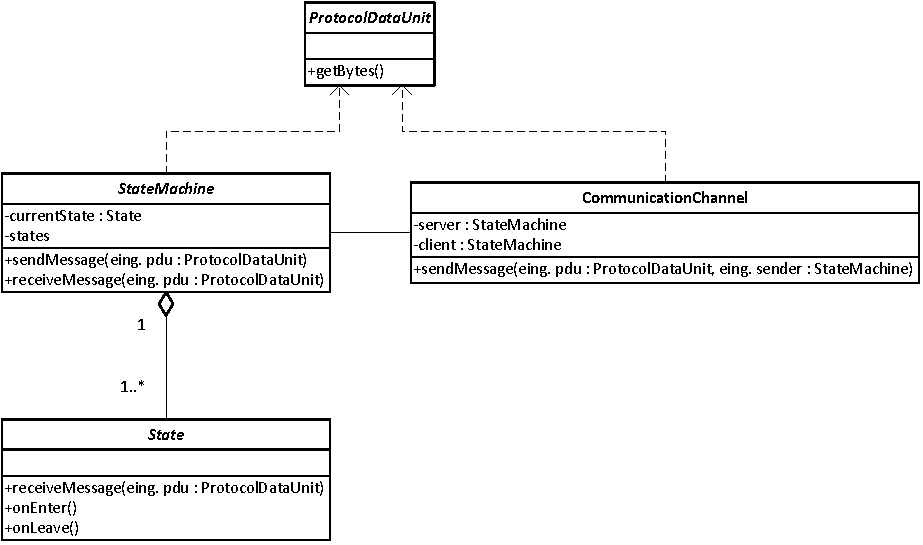
\includegraphics[scale=0.9]{Diagrams/uml/abstract_pdu_state_machine_channel.pdf} %scale=0.8
	\caption{UML-Diagramm der Umsetzung des abstrakten Rahmens}
	\label{fig_uml_abstract_state_machine}
\end{figure}

Für die Übertragung von Nachrichten wird ein \sourceobject{CommunicationChannel}-Objekt genutzt, dass die Übermittlung von Nachrichten zwischen den beiden an dem Protokollablauf beteiligten \sourceobject{StateMachine}-Objekten übernimmt. Außerdem ist in diesem Objekt auch die Thread-Synchronisierung implementiert, die dafür sorgt, dass der Protokollablauf beim Senden einer Nachricht pausiert wird. Dies ermöglicht das schrittweise Verfolgen der gesendeten Nachrichten und der Veränderungen des internen Zustands der Kommunikationspartner. Auch \sourceobject{CommunicationChannel}-Objekte können beobachtet werden, um über zu sendende oder gesendete Nachrichten informiert zu werden.

Um Protokollerweiterungen eine typsichere Umgebung zu bieten, besitzen die \sourceobject{StateMachine}-, \sourceobject{State}- und \sourceobject{CommunicationChannel}-Klassen einen generischen Parameter vom Typ einer Unterklasse von \sourceobject{ProtocolDataUnit}. Hierdurch können Unterklassen ihren Nachrichtentyp angeben und sich auf die durch Java gewährleistete Typsicherheit verlassen.
\todo{listing of headers?}

% abstract view

Für die Darstellung des Protokollablaufs wurde ein Gerüst entwickelt, das die im vorherigen Abschnitt beschriebenen Gemeinsamkeiten von Protokollen abbildet. Für die internen Zustände der Parteien werden zwei Bereiche angelegt, die durch konkrete Protokolle bereitgestellt werden müssen. Außerdem wird eine Liste von bereits gesendeten bzw. als nächstes gesendeten Nachrichten angezeigt, die es ermöglicht bei Auswahl einer Nachricht Details zu dieser anzuzeigen. Dabei wird für jede Nachricht die Darstellung als Bytekette und eine protokollspezifische Detailansicht, die ebenfalls durch konkrete Protokolle bereitgestellt werden muss, angeboten. Zusätzlich kann ein weiteres Fenster angezeigt werden, dass es ermöglicht Informationen zu gewünschten zustands- oder nachrichtenabhängigen Daten anzubieten.\\
Für die Interaktion wird ein Bedienfeld angezeigt, dass die Nachrichtensteuerung bereitstellt und das Informationsfenster öffnet. In der Nachrichtendetaildarstellung können die Bytes einer Nachricht vor dem Senden verändert werden.\\
Für die Verknüpfung der Datenschicht mit der Benutzeroberfläche wurde das Entwurfsmuster Model-View-Presenter (siehe \cite{potel96}) gewählt, um eine strukturierte Trennung der Schichten zu ermöglichen.

% abstract provider and builder

Um Erweiterungen die Bereitstellung fehlender Elemente und nötiger Objekte zu ermöglichen, wurden die Interfaces \sourceobject{ViewProvider} und \sourceobject{StateMachineProvider} erstellt, die eine Erweiterung implementieren muss. Objekte, die diese Interfaces implementieren, ermöglichen es das Gerüst mit protokollspezifischen Details zu füllen. \sourceobject{ViewProvider} sorgen für die Bereitstellung von Fensterelementen für die internen Zustände der Parteien, für die Detailansicht einer Nachricht und für optionale Einstellmöglichkeiten zu dem Protokollablauf. \sourceobject{StateMachineProvider} sind zuständig für die entsprechenden \sourceobject{StateMachine}-Objekte für die beiden Parteien. Diese werden dann durch einen \sourceobject{ProtocolBuilder} mit einem \sourceobject{CommunicationChannel} und den entsprechenden Fensterelementen verknüpft. In Abbildung \ref{fig_uml_abstract_provider_builder} ist ein UML-Diagramm zu finden, das diese Zusammenhänge visualisiert. 

\begin{figure}
	\centering
	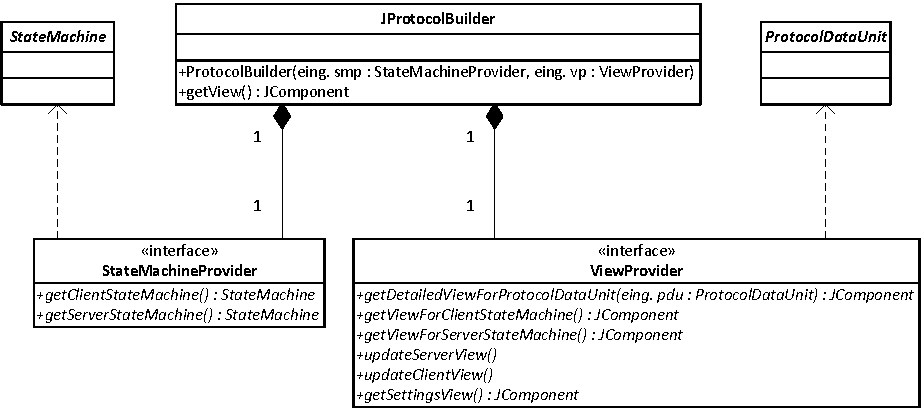
\includegraphics[scale=0.9]{Diagrams/uml/abstract_provider_builder.pdf} %scale=0.8
	\caption{UML-Diagramm von Provider- und ProtocolBuilder-Klassen für die Bereitstellung von Erweiterungen}
	\label{fig_uml_abstract_provider_builder}
\end{figure}

Beim Laden einer neuen Protokollsimulation wird eine Liste vorhandener Protokolle und bei Auswahl eines Eintrags die entsprechende Einstellungsansicht angezeigt. Wenn eine Protokollsimulation gestartet wird, wird das vom \sourceobject{ProtocolBuilder} zur Verfügung gestellte Fensterelement in die Anwendung eingebettet.

\subsection{Erweiterung der Anwendung um TLS 1.2}

% tls 12 model

	% TlsCiphertext and included fragment/message
Als Protokollnachricht dient die Klasse \sourceobject{TlsCiphertext}. Bei ihrer Modellierung wurde versucht analog zu der Spezifikation vorzugehen und auch Benennungen möglichst einheitlich zu halten. Sie enthält Felder für den \sourceobject{TlsContentType}, die \sourceobject{TlsVersion} und ihre Länge, sowie ein \sourceobject{TlsFragment}, das die eigentliche Nachricht der oberen TLS-Protokollschicht enthält. \\
Abhängig von der aktuellen \ciphersuite{} wird dieses \sourceobject{TlsFragment} verschlüsselt und mit einem MAC versehen und enthält weitere Felder für bei der Verschlüsselung benötigte Werte (siehe Abschnitt \ref{sec_record_protocol} und insbesondere Abbildung \ref{fig_tls_cipher_types}). \\
Die Nachrichten der oberen Schicht werden durch für jedes Teilprotokoll bestehende Unterklassen von \sourceobject{TlsMessage} dargestellt. Neben \sourceobject{TlsAlertMessage}, \sourceobject{TlsChangeCipherSpecMessage} und \sourceobject{TlsApplicationDataMessage} wurde für jeden HandshakeType eine eigene Klasse erstellt. Alle diese Nachrichten enthalten zwei Konstruktoren, die die Erstellung aus benötigten Werten und die Erstellung durch das Parsen übertragener Bytes ermöglichen. 

	%state machine, states, security paramaters, connection state

Im Folgenden werden die implementierten Klassen für das TLS-Automatenmodell beschrieben. Ein UML-Diagramm ist in Abbildung \ref{fig_uml_tls_state_machine} zu finden.

Als Unterklasse der \sourceobject{StateMachine}-Klasse wurde \sourceobject{TlsStateMachine} implementiert. Diese Klasse bietet Zugriff auf alle notwendigen, internen Zustandsinformationen von TLS-Client und -Server. Ein Objekt vom Typ \sourceobject{TlsSecurityParameters} bietet Zugriff auf während des Handshakes ausgehandelte Verfahren und Informationen wie SessionId, Random-Werte und das berechnete \mastersecret{}. Objekte vom Type \sourceobject{TlsConnectionState} bilden den current read und write state, sowie den pending state (vgl. Abschnitt \ref{sec_change_cipher_spec}). In ihnen werden ausgehandelte \ciphersuite{} und Schlüssel sowie die aktuelle Sequenznummer verwaltet. Bei Empfang oder nach dem Senden einer \changecipherspec{}-Nachricht kann der pending state zum current state gemacht werden.\\
Für Client und Server wurde jeweils eine Unterklasse \sourceobject{TlsClientStateMachine} und \sourceobject{TlsServerStateMachine} erstellt, die unterschiedliches Verhalten der beiden Parteien enthalten. Insbesondere im Bereich der asymmetrischen Kryptographie sind diese Unterschiede so groß, dass der Mehraufwand gerechtfertigt ist. Beispielsweise besitzt der Server ein RSA-Schlüsselpaar, dessen geheimer Schlüssel zum Entschlüsseln des vom Client ausgewählten \premastersecret{} oder zum Signieren der Diffie-Hellman-Parameter genutzt wird. Der Client ist im Gegensatz dazu lediglich im Besitz des öffentlichen Serverschlüssels zum Verschlüsseln des \premastersecret{}s oder zum Überprüfen der Parametersignatur.

\begin{figure}
	\centering
	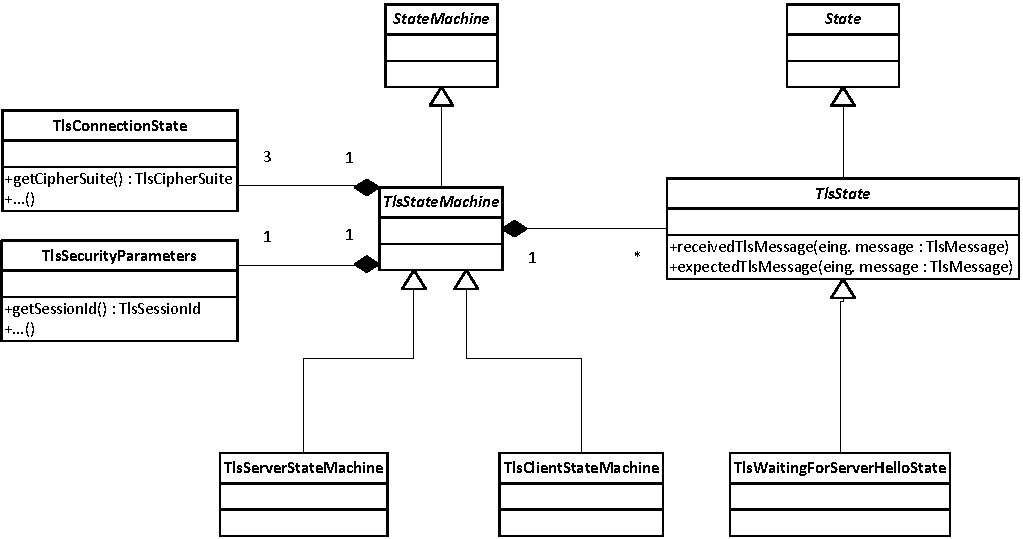
\includegraphics[scale=0.9]{Diagrams/uml/tls_state_machine.pdf} 
	\caption{UML-Diagramm der Klassen für das Tls-Automatenmodell}
	\label{fig_uml_tls_state_machine}
\end{figure}

Entsprechend den Automatenmodellen im Anhang \ref{cha_tls_state_machines} wurden für alle Zustände entsprechende Unterklassen von \sourceobject{TlsState}, einer Unterklasse von \sourceobject{State}, erstellt. Jede dieser Unterklassen definiert die Typen von TLS-Nachrichten der oberen Schicht, die sie erwartet, und implementiert das Verhalten bei Empfang einer solchen Nachricht. Beispielsweise erwartet der Clientzustand \sourceobject{TlsWaitingForServerHelloState} lediglich Handshake-Nachrichten vom Typ \serverhello{}. Bei Empfang einer solchen Nachricht werden die entsprechenden Felder für TlsVersion, ServerRandom, SessionID und \ciphersuite{} gesetzt und der aktuelle Zustand der \sourceobject{TlsClientStateMachine} auf den nachfolgenden Zustand gesetzt. Diese Umsetzung ist in Listing \ref{lst_state_example} zu finden. Nach dem gleichen Prinzip wird das Verhalten in allen anderen Zuständen implementiert. 

\lstset{style=java, caption={Implementierung des Zustands \sourceobject{TlsWaitingForServerHelloState}}, label=lst_state_example}
\begin{lstlisting}
public class TlsWaitingForServerHelloState extends TlsState {
	...
	%%@Override%%
	public boolean expectedTlsMessage(TlsMessage message) {
		return isHandshakeMessageOfType(message, TlsHandshakeType.server_hello);
	}

	%%@Override%%
	public void receivedTlsMessage(TlsMessage message) {
		...
		setServerHelloValues(message);
		setTlsState(TlsStateType.CLIENT_IS_WAITING_FOR_CERTIFICATE_STATE)
	}

	private void setServerHelloValues(TlsServerHelloMessage message) {
		...
		_stateMachine.setVersion(version);
		_stateMachine.setServerRandom(message.getServerRandom());
		_stateMachine.setSessionId(message.getSessionId());
		_stateMachine.setPendingCipherSuite(message.getCipherSuite());
	}
}
\end{lstlisting}

In der Oberklasse \sourceobject{TlsState} werden eingehende Nachrichten entschlüsselt. Dieser Vorgang wird in den folgenden Absätzen näher beleuchtet. Danach werden die Nachrichten je nach gesetztem ContentType geparst. Fehler bei diesem Vorgang führen zu einem Übergang in einen Fehlerzustand und Senden einer Alert-Nachricht. Anschließend wird überprüft, ob die geparste Nachricht von dem aktuellen Zustand erwartet wird. Ist dies nicht der Fall, so wird ebenfalls ein Fehlerzustand gesetzt und eine Alert-Nachricht gesendet.

	%crypto cipher suites
Im TLS-Protokoll werden die verwendeten Algorithmen und Schlüssellängen durch \ciphersuites{} zur Verfügung gestellt (siehe Abschnitt \ref{sec_cipher_suites}). Durch das Interface \sourceobject{TlsCipherSuite} werden diese Werte zu Verfügung gestellt. Für die Anwendung wurden verschiedene \sourceobject{TlsCiphersuite}-implementierende Klassen entwickelt, die verschiedene Algorithmen zum Schlüsselaustausch und zur Verschlüsselung beinhalten:
\begin{itemize}
\item TLS\_DHE\_RSA\_WITH\_AES\_128\_CBC\_SHA
\item TLS\_DHE\_RSA\_WITH\_AES\_128\_GCM\_SHA256
\item TLS\_RSA\_WITH\_AES\_128\_CBC\_SHA
\item TLS\_RSA\_WITH\_AES\_128\_GCM\_SHA256
\end{itemize}
Durch diese Wahl der \ciphersuites{} können sowohl der Diffie-Hellman- als auch der RSA-Schlüsselaustausch beobachtet werden. Außerdem ist die Verschlüsselung per Blockchiffre (AES im CBC-Modus) oder AEAD-Chiffre (AES im GCM-Modus) möglich. \\
Für die kryptographischen Algorithmen wurde auf die Implementierungen der Java-Bibliothek zurückgegriffen. Die TLS-spezifische PseudoRandomFunction wurde eigenständig entwickelt und durch Testvektoren auf ihre Richtigkeit hin überprüft. Ebenso wurde auch die Verknüpfung der Algorithmen für die Ver- und Entschlüsselung, also beispielsweise die Berechnung von MAC, Padding und Paddinglänge und die anschließende Verschlüsselung, für Block- und AEAD-Chiffren selber in den Klassen \sourceobject{TlsBlockCipherSuite} und \sourceobject{TlsAeadCipherSuite} implementiert. Konkrete \ciphersuites{} füllen lediglich die vorgegebenen Rahmen und bieten Zugriff auf Schlüssellängen und die verwendeten Algorithmen.

In der \sourceobject{TlsState}-Klasse werden zu sendende Nachrichten durch die im current write state gesetzte \ciphersuite{} von \sourceobject{TlsPlaintext}- in \sourceobject{TlsCiphertext}-Objekte umgewandelt und anschließend gesendet. Beim Empfang von Nachrichten wird dieser Prozess umgekehrt durchlaufen. Bei auftretenden Fehlern wie einem falschen Schlüssel oder einem ungültigen MAC erfolgt wiederum der Übergang in einen Fehlerzustand und das Senden einer Alert-Nachricht.

% tls 12 view

Für die Benutzeroberfläche wurde den Überlegungen im vorherigen Abschnitt entsprechend für Client und Server ein auf der Swing-Komponente \sourceobject{JTree} basierendes Fensterelement entwickelt. Der interne Zustand der Parteien wird durch Titel-Wert-Paare und optionale Kindelemente dargestellt. Die Klasse \sourceobject{TlsStateMachine} enthält eine Methode, die die Paare für den aktuellen Zustand zurückliefert. Bei Zustandsänderungen, die durch das Beobachter-Muster kommuniziert werden, werden der alte und neue Zustand verglichen und neue oder geänderte Einträge gekennzeichnet, sodass Auswirkungen von empfangenen Nachrichten sichtbar werden. Zusätzlich wurde zu den jeweiligen Einträgen jeweils ein erklärender Informationstext mit Auszügen aus der Spezifikation erstellt, um ein besseres Verständnis der Abläufe zu unterstützen.\\
Zusätzlich enthalten die Fensterelemente Buttons für die verfügbaren Aktionen wie das Verbinden oder das Senden von Daten bei bestehender Verbindung.

Das gleiche Fensterelement wie für Server und Client wurde auch für die Detaildarstellung von Nachrichten verwendet. Auch für die jeweiligen Nachrichtenfelder wurden Informationstexte erstellt, die beim Verstehen der Protokolls helfen sollen.

\begin{figure}
	\centering
	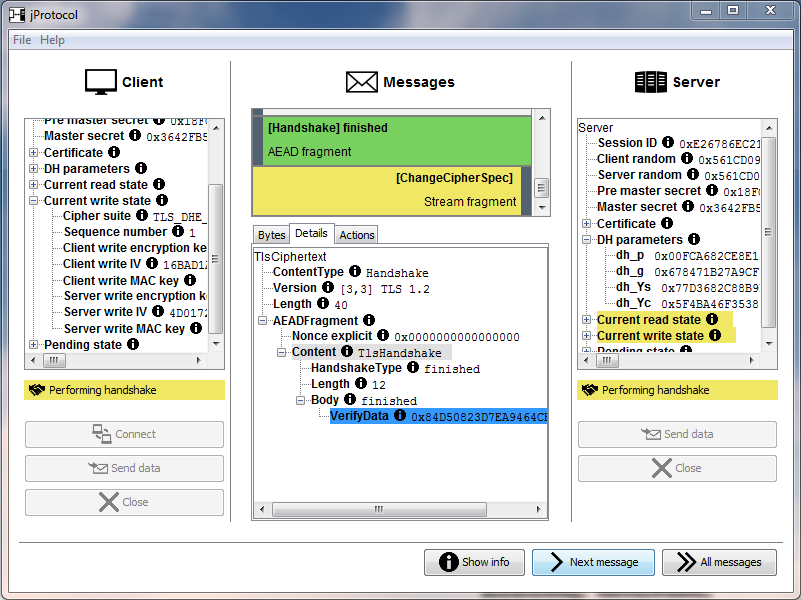
\includegraphics[scale=0.7]{Diagrams/ScreenshotTLS.png} 
	\caption{Die fertige Anwendung}
	\label{fig_application_screenshot}
\end{figure}

Ein Screenshot der endgültigen Anwendung mit der Erweiterung um TLS ist in Abbildung \ref{fig_application_screenshot} zu finden.

\section{Erweiterung der Anwendung}

In diesem Abschnitt soll anhand eines einfachen Beispiels gezeigt werden, was bei der Erweiterung der Anwendung um ein weiteres Protokoll zu beachten ist. Dazu wird ein einfaches Protokoll betrachtet, bei dem eine Nachricht lediglich aus einem Längenfeld und einem Nachrichteninhalt besteht. Ein Client kann Nachrichten dieses Formats an den Server senden, der diese lediglich genauso zurücksendet. Es handelt sich also um eine leicht modifizierte Variante des Echo-Protokolls\footnote{Das Echo-Protokoll wird in RFC 862 spezifiziert.}.

Im ersten Schritt wird der Nachrichtentyp implementiert (siehe Listing \ref{lst_echo_message}).

\lstset{style=java, caption={Implementierung des Nachrichtentyps \sourceobject{EchoMessage}}, label=lst_echo_message}
\begin{lstlisting}
public class EchoMessage extends ProtocolDataUnit {
	
	private String _messageContent;
	...
	%%@Override%%
	public byte[] getMessageBytes() {
		byte[] lengthBytes = ByteHelper.intToByteArray(getLength());
		byte[] messageContentBytes = _messageContent.getBytes(StandardCharsets.US_ASCII);
		return ByteHelper.concatenate(lengthBytes, messageContentBytes);
	}

	%%@Override%%
	public String getTitle() {
		return "Echo message";
	}

	%%@Override%%
	public String getSubtitle() {
		return _messageContent;
	}
}
\end{lstlisting}

Anschließend werden Automaten für Server und Client entwickelt. Dazu wird die Klasse \sourceobject{StateMachine} mit dem formalen Typparameter \sourceobject{EchoMessage} erweitert. Für die Automaten müssen von \sourceobject{State} abgeleitete Zustände entwickelt werden, die das Verhalten abbilden. In diesem einfachen Beispiel genügt ein Zustand für den Server, in dem empfangene Nachrichten unverändert wieder gesendet werden (siehe Listing \ref{lst_echo_server_state_machine}). Analog ist für den Client vorzugehen. Der Client benötigt jedoch zusätzlich noch eine Methode \sourceobject{sendEchoRequest()}, um Nachrichten an der Server senden zu können. Außerdem wurden, um den Zustandswechsel zu demonstrieren, ein Sende- und ein Empfangszustand implementiert. 

\begin{lstlisting}[style=java, caption={Implementierung des Serverautomaten}, label=lst_echo_server_state_machine]
public class EchoServer extends StateMachine<EchoMessage> {

	public final Integer RECEIVE_STATE = 1; 
	
	public EchoServer() {
		addState(RECEIVE_STATE, new ReceiveState(this));               
		setState(RECEIVE_STATE);
	}
}

public class ReceiveState extends State<EchoMessage> {

	public ReceiveState(EchoServer stateMachine) {
		super(stateMachine);
	}

	%%@Override%%
	public void receiveMessage(EchoMessage pdu) {
			EchoMessage echo = new EchoMessage(pdu.getMessageContent());
			sendMessage(echo);
	}
}
\end{lstlisting}

Danach wird eine Klasse \sourceobject{EchoProvider} erstellt, die der Anwendung Zugriff auf die Automaten für Server und Client, sowie auf zu implementierende Fensterelemente bietet. Außerdem muss sich die Klasse auch um die Aktualisierung der Fensterelemente bei Änderung des internen Zustand von Server oder Client kümmern. Diese Klasse muss die Interfaces \sourceobject{ViewProvider} und \sourceobject{StateMachineProvider} implementieren (siehe Listing \ref{lst_echo_provider}).

\begin{lstlisting}[style=java, caption={Implementierung der \sourceobject{EchoProvider}-Klasse}, label=lst_echo_provider]
public class EchoProvider implements ViewProvider<EchoMessage>, StateMachineProvider<EchoMessage> {

	%%@Override%%
	public StateMachine<EchoMessage> getServerStateMachine() {
		return new EchoServer();
	}
	...
}
\end{lstlisting}

Für den Server wird lediglich ein leeres Fensterelement erzeugt, für den Client eine Liste mit empfangenen Serverantworten sowie ein Button, um neue Anfragen abzuschicken. Zwei Dinge sind hier zu beachten.\\
Methoden, die aus dem UI-Thread (also beispielsweise bei Drücken eines Buttons) aufgerufen werden und dazu führen, dass eine neue Nachricht gesendet wird, müssen zwingend in einem neuen Thread aufgerufen werden, um das erfolgreiche Pausieren bei einer Nachrichtenübertragung zu ermöglichen. Die Umsetzung für den Echo-Client ist in Listing \ref{lst_echo_button_thread} zu finden.

\lstset{style=java, caption={Starten eines neuen Threads für das Senden einer Nachricht}, label=lst_echo_button_thread}
\begin{lstlisting}
JButton sendButton = new JButton("Send...");
sendButton.addActionListener(new ActionListener() {
	%%@Override%%
	public void actionPerformed(ActionEvent e) {
		new Thread(new Runnable() {
			@Override
			public void run() {
				_client.sendEchoRequest("DATEN!");
			}
		}).start();
	}
});
\end{lstlisting}

Außerdem kann ein bereits implementierter Mechanismus dazu genutzt werden, auf Zustandsänderungen von Server oder Client zu reagieren. Dazu muss lediglich die Methode \sourceobject{notifyObserversOfStateChanged()} aus einem Zustand heraus aufgerufen werden. Dies führt zur Ausführung von \sourceobject{updateServerView} bzw. \sourceobject{updateClientView} des \sourceobject{EchoProvider}-Objekts, in dem die erstellten Fensterelemente aktualisiert werden können. In der \sourceobject{updateClientView}-Methode der \sourceobject{EchoProvider}-Klasse wird beispielsweise die Liste der bisher empfangenen Serverantworten aktualisiert (siehe Listing \ref{lst_echo_state_changed}).

\begin{lstlisting}[style=java, caption=Aktualisierungsmechanismus bei Zustandsänderung, label=lst_echo_state_changed]
class ReceiveState extends State<EchoMessage> {
	...
	%%@Override%%
	public void receiveMessage(EchoMessage pdu) {
		_receivedMessages.add(pdu.getPayload());
		_stateMachine.notifyObserversOfStateChanged();

		setState(SEND_STATE);
	}
}

public class EchoProvider implements ... {
	...
	%%@Override%%
	public void updateClientView() {
		_clientTextArea.setText("");
		for (String text : _client.getReceivedMessages()) {
			_clientTextArea.append(text + "\n");
		}
	}
}
\end{lstlisting}

Als letztes muss das entwickelte Protokoll noch in der Anwendung einzutragen. Dazu muss der Protokollliste in der Klasse \sourceobject{ProtocolRegistry} noch ein \sourceobject{JProtocolBuilder}-Objekt hinzugefügt werden (siehe Listing \ref{lst_echo_protocol_registry}).

\begin{lstlisting}[style=java, caption=Protokollregistrierung, label=lst_echo_protocol_registry]
public class ProtocolRegistry {
	...
	public ProtocolRegistry() {
		...
		EchoProvider echoProvider = new EchoProvider();
		_protocolMap.put("EchoProtocol", new ProtocolBuilder<>(echoProvider, echoProvider));
	}	
}
\end{lstlisting}

Ein abschließender Hinweis: Für die Darstellung von Client, Server und den Details einer Nachricht kann auch die in dem entwickelten TLS-Plugin verwendete Baumstruktur verwendet werden, die als Klasse \sourceobject{KeyValueTree} verfügbar ist.